\chapter{Complementarity with Other Experiments}
\Contributors{Josh S., Ting L., Will, Andrew P. Manuel, Chanda, Alex, many others ...}
\label{sec:complementarity}
\bigskip

The LSST data set will uniquely complement many other experimental studies of dark matter.
Below we summarize some of these complementary probes, with a specific focus on spectroscopic observations, high resolution imaging, indirect detection experiments, and direct detection experiments.
While LSST can substantial improve our understanding of dark matter in isolation, support of these experiments is essential to provide an comprehensive picture of dark matter physics.
This section is not intended to be comprehensive, but rather serves to demonstrate the influence that LSST will have on dark matter studies generally.

% Spectroscopy
\section{Spectroscopy \Contact{Ting}}
 \Contributors{Josh S., Ting L., Erik T., ...}
 \label{sec:spectroscopy}

%(TL: do we want to make a table to compare the specs of various spectroscopy facility. I do not think this is the scope of this paper...) ADW: I agree, this seems beyond our scope%\TL{need to check if ESO wide-field instrument has a name already or not}

While the photometric and astrometric measurements from LSST alone are quite powerful, their impact can be significantly augmented by additional spectroscopic observations. 
In particular, spectroscopic follow-up studies will provide kinematic and redshifts information for many of the objects studied by LSST.
Given the faintness and high density of targets that are expected from LSST, community access to multi-object spectrograph on large aperture telescopes is essential for these studies \citep{2016arXiv161001661N}. 
Due to LSST's location in the southern hemisphere, southern spectroscopic facilities are best, as this  maximizes the overlapping sky area.

Many next-generation telescopes and instruments are currently under preparation or construction. These instruments are broadly divide into two categories: massively multiplexed spectrographs on 8 to 10-meter telescopes, and giant segmented mirror telescopes (GSMTs, $\sim30$-meter class) with smaller field of view. The former category includes facilities on exisiting and future telescopes including the Southern Spectroscopic Survey Instrument (SSSI), a project recommended for consideration by the DOE’s Cosmic Visions panel \citep{1604.07626, 1604.07821}, the Primary Focus Spectrograph (PFS) instrument on the Subaru telescope \citep{2014PASJ...66R...1T}, the Maunakea Spectroscopic Explorer \citep[MSE;][]{MSEbook2018}, and a possible future ESO wide-field spectroscopic facility. 
The latter category is populated by new facilities such as Thirty Meter Telescope \citep[TMT;][]{1505.01195}, the Giant Magellan Telescope \citep[GMT;][]{GMT:2018}, and the European Extremely Large Telescope \citep[E-ELT;][]{EELT:2009}. 

In this section, we illustrate several examples of how complementary spectroscopy will improve the measurements on the dark matter properties with LSST.

\subsection{Milky Way Dwarfs \Contact{Josh}}
\Contributors{Josh, Ting, Erik, ...}
In Section~\ref{sec:smallest_galaxies} we discussed the derivation of an upper limit on the minimum dark matter halo mass based only on the observed luminosity function of satellites discovered by LSST. \ET{Should we mention the fact that confirmation of the LSST discoveries *also* may require spectroscopy at least for some of the ambiguous cases?}  An alternative approach is to obtain spectroscopy of individual stars in each satellite to measure its velocity dispersion, from which the central mass and density can be inferred.  Then one can compare either the densities or the circular velocity function directly with theoretical predictions without assumptions about the subhalo mass function or the stellar mass-halo mass relation.

Spectroscopy of individual stars in the faint Milky Way satellites that will be identified with LSST will require deep observations with multiplexed spectrographs on large telescopes.  Measurements of the stellar velocity dispersions of these systems can be obtained either with 8-10~m-class telescopes or with the next generation of 25-30~m telescopes.  As illustrated in Fig.~\ref{fig:specfollowup_distance}, spectroscopy of a nearly complete sample of satellites can be pushed $\sim2$~mag fainter in luminosity and a factor of $\sim2$ farther in distance with plausible investments of observing time on a GSMT than with existing facilities.

In additional to inferring the minimum dark matter halo mass, kinematics from stellar spectroscopy can also reveal the density profile of the dwarf galaxies at the lowest luminosities, in which the baryonic effects are minimum and therefore dark matter physics can be separated from the astrophysics of galaxy formation (cite). A direct measurement of the density profile in these dwarf galaxies will allow us to distinguish between collisionless CDM  which predicts a cusp NFW profile, and SIDM which predicts a core profile (cite). Moreover, the stellar kinematics will also reveal the integral of the dark matter density profile in the dwarf galaxy (or J-factor), which is an essential input for the constraints on the dark matter self-annihilation cross section for the indirect dark matter search in X-ray and gamma-ray experiments \citep[e.g.][]{1108.3546}.


\begin{comment}
\begin{figure}
\centering
\vspace{-2in}
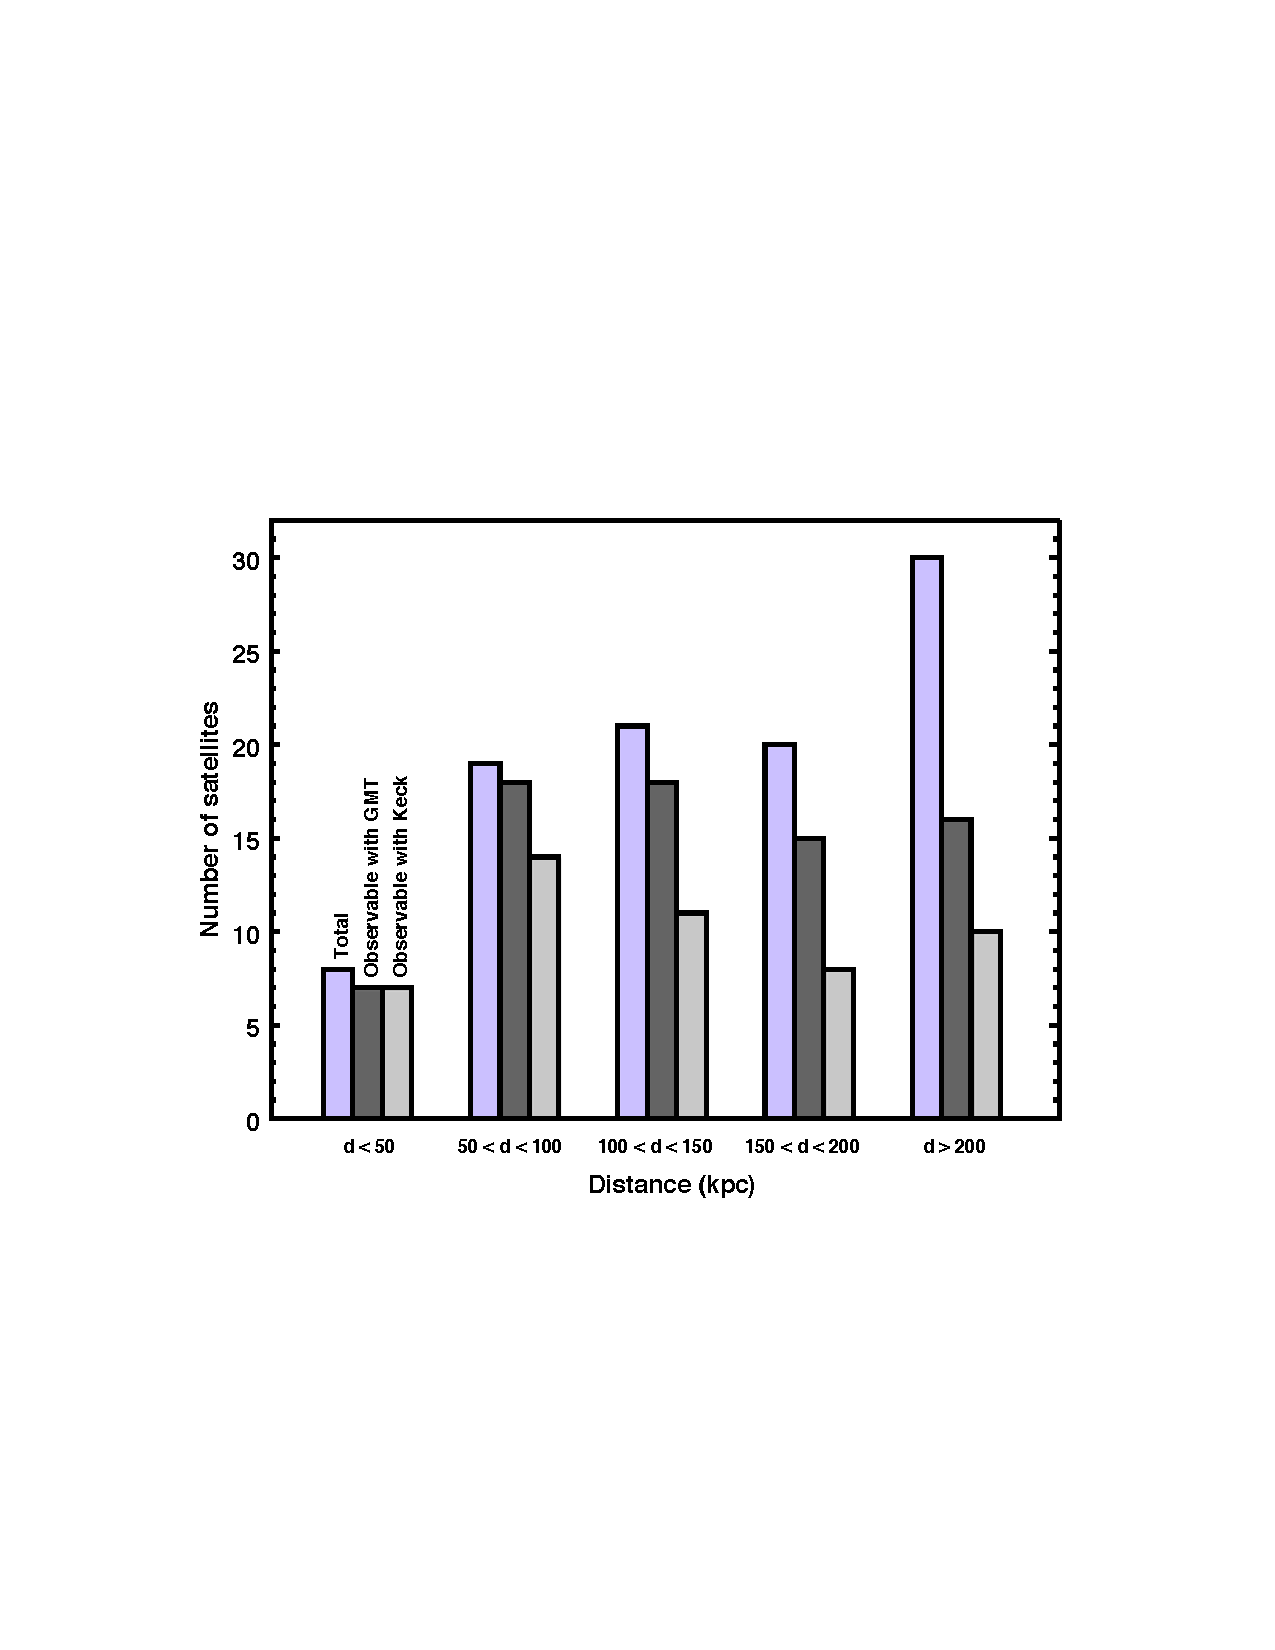
\includegraphics[width=0.85\textwidth]{figures/dwarf_observability_barplot_distance.pdf}
\vspace{-2in}
\caption{Possibility of spectroscopic follow-up for the LSST satellite population as a function of distance. Current telescopes will be able to measure velocity dispersions for $\sim50\%$ of the expected satellites, while a GSMT can measure velocity dispersions for $\sim80\%$. }\label{fig:specfollowup_distance}
\end{figure}


\begin{figure}
\centering
\vspace{-2in}
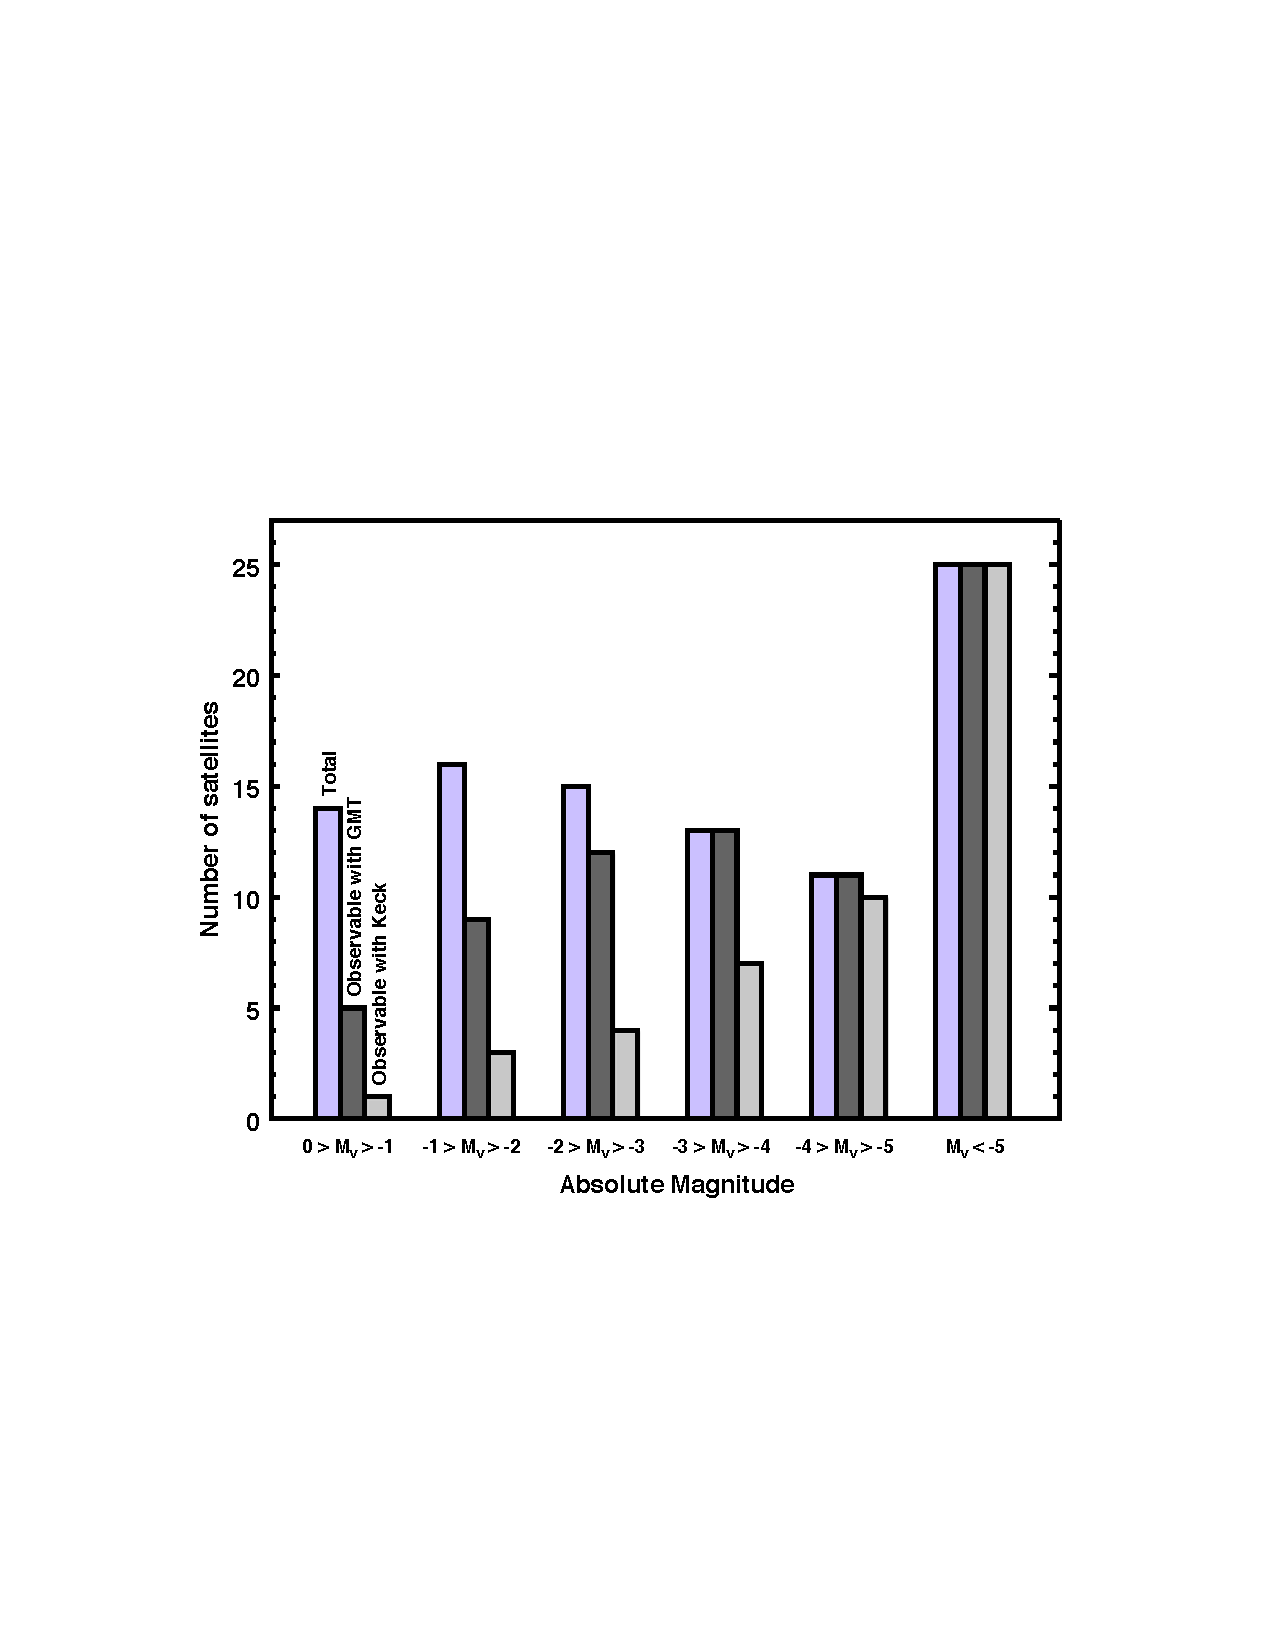
\includegraphics[width=0.85\textwidth]{figures/dwarf_observability_barplot_luminosity.pdf}
\vspace{-2in}
\caption{Possibility of spectroscopic follow-up for the LSST satellite population as a function of magnitude. }\label{fig:specfollowup_distance}
\end{figure}
\end{comment}

\begin{figure}
  \centering
  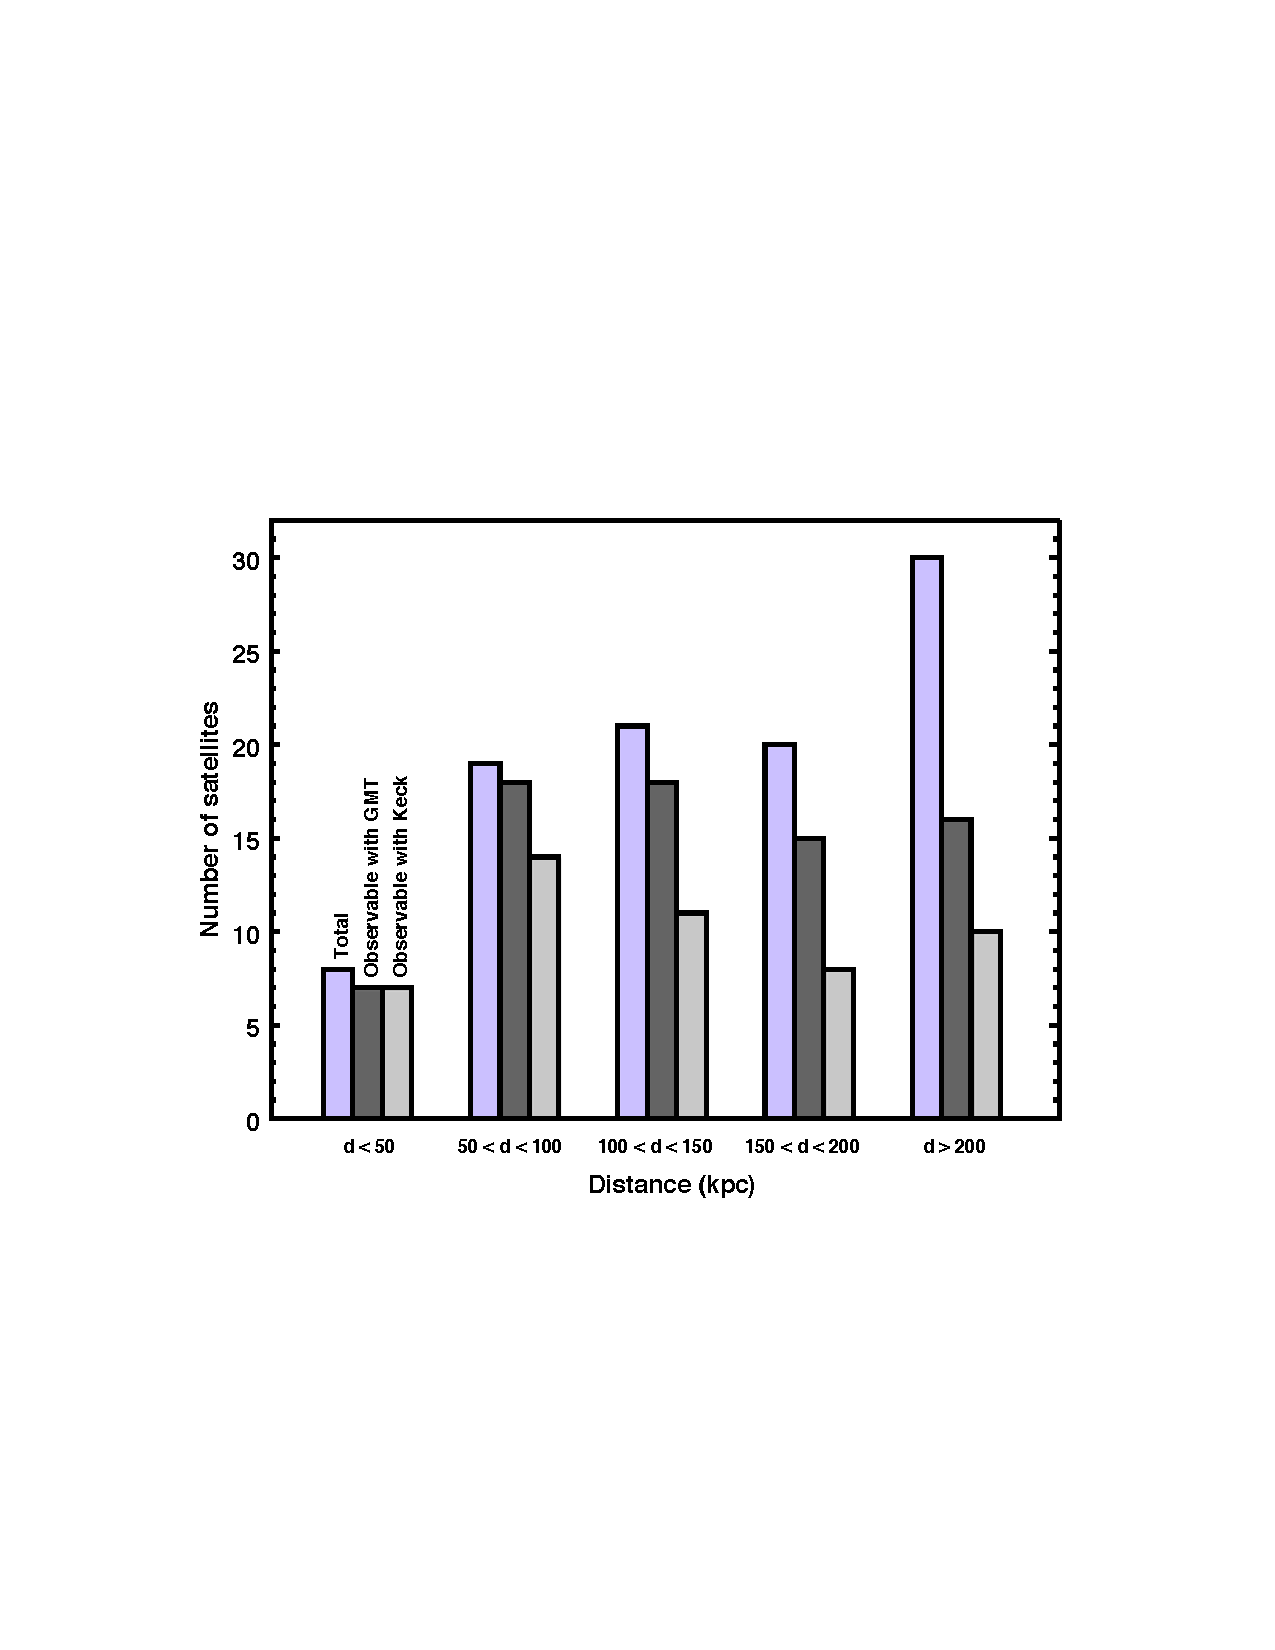
\includegraphics[width=0.49\textwidth]{figures/dwarf_observability_barplot_distance.pdf}
  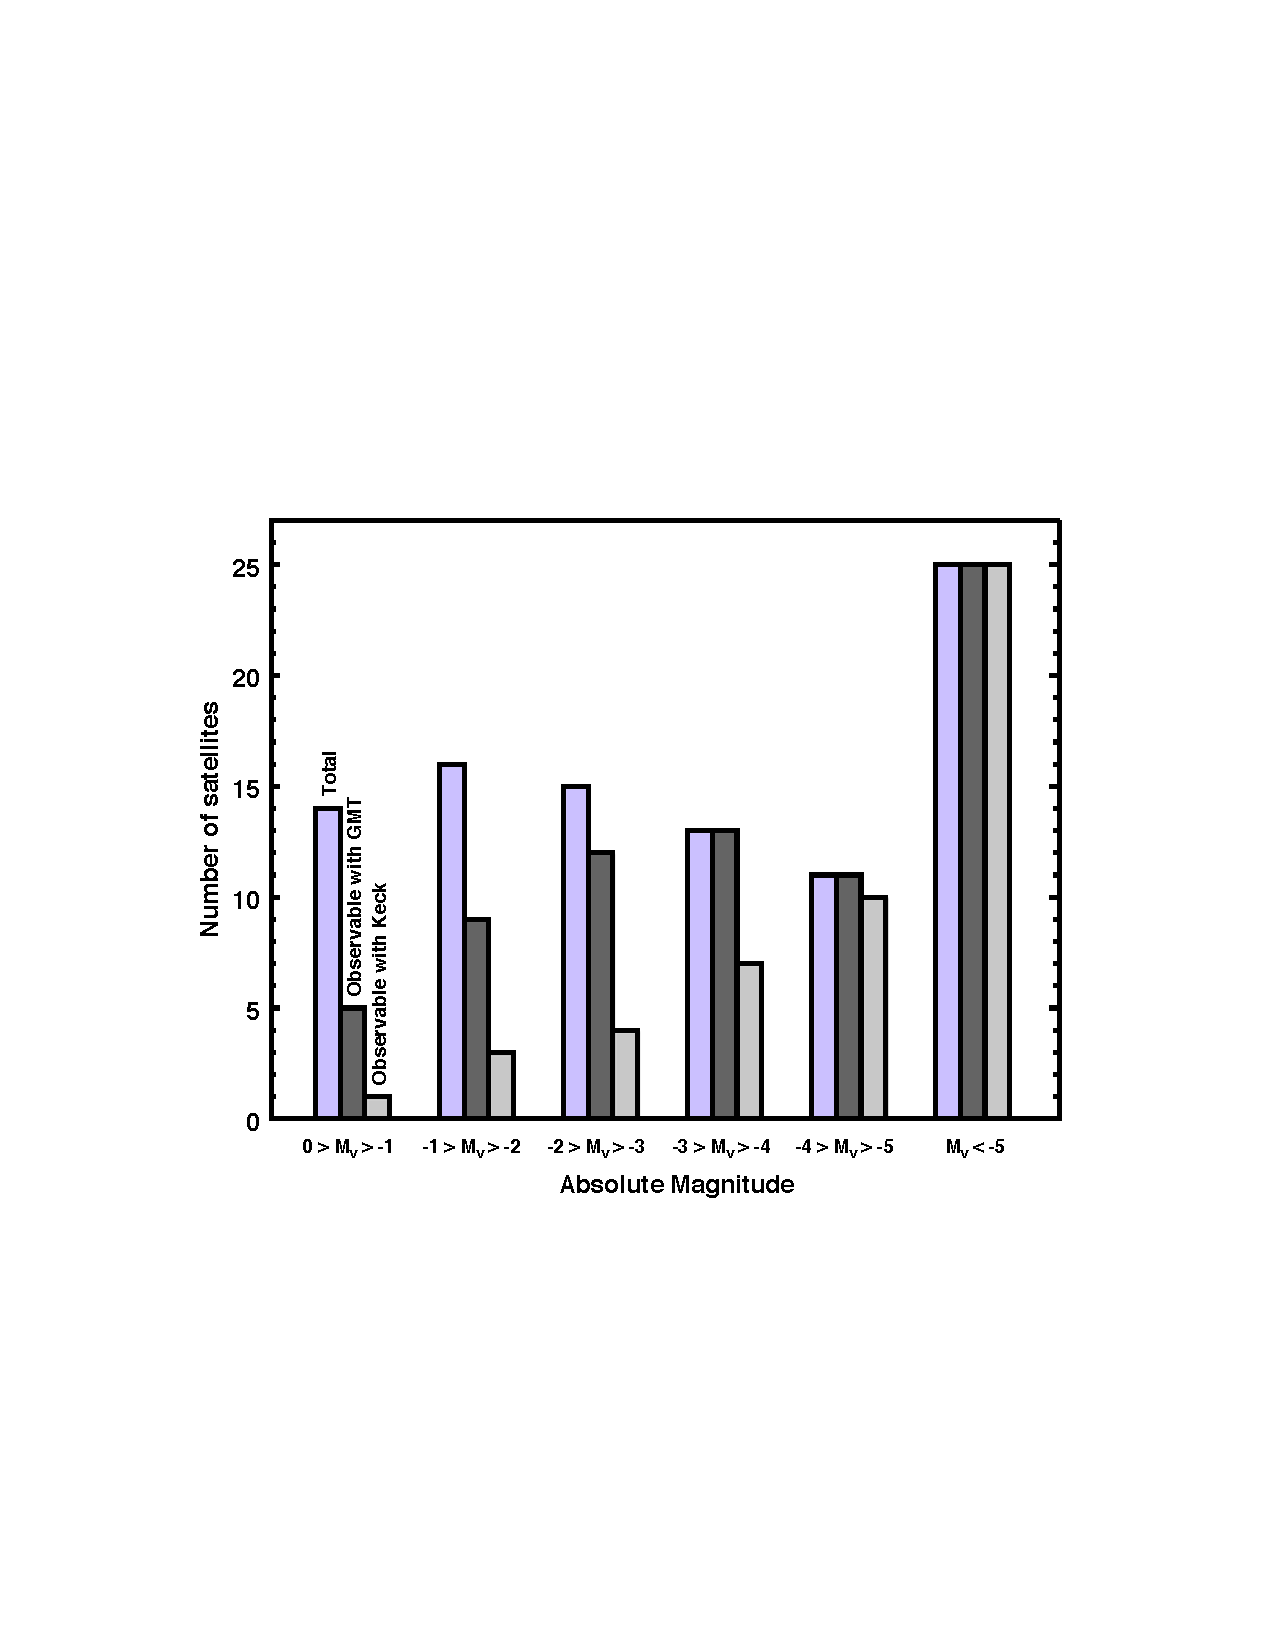
\includegraphics[width=0.50\textwidth]{figures/dwarf_observability_barplot_luminosity.pdf}
  \caption{Possibility of spectroscopic follow-up for the LSST satellite population as a function of distance (left) and magnitude (right). Current telescopes will be able to measure velocity dispersions for $\sim50\%$ of the expected satellites, while a GSMT can measure velocity dispersions for $\sim80\%$.}
  \label{fig:specfollowup_distance}
\end{figure}

\subsection{Stellar Streams \Contact{Ting}}
\Contributors{Ting, Denis ...}

As discussed in Section~\ref{sec:stream_gaps}, subhalo encounters with cold stellar streams will induce density perturbations that will be detectable by LSST, constraining the minimum dark matter halo mass and the mass function of dark matter halos from $\sim10^{5} - 10^{9}$~M$_{\odot}$. In addition, these flybys cause velocity perturbations that correlate with the density variations.  The velocity signal near stream gaps can be measured either via line-of-sight velocity measurements from spectroscopy or tangential velocity measurements from astrometry, improving the precision with which the perturber mass can be determined.
The velocity variation (peak to peak) from these flybys will be small. To estimate the amplitude of the perturbation, we consider a stream orbiting the Milky Way at a distance of 14 kpc and compute the typical maximum velocity kick expected over its lifetime of 5 Gyr using the formalism from \cite{erkal2016}.  The velocity change is $\sim$0.6, 0.3, 0.1 km/s for subhalos in the range $10^7-10^8 M_\odot$, $10^6-10^7 M_\odot$, $10^5 -10^6 M_\odot$ respectively. Due to the low density of the stream stars, a massively multiplexed, wide field-of-view spectroscopic facility such as PFS on Subaru or MSE is needed. Furthermore, given the expected small velocity kick amplitude, the velocity accuracy for each star determined from the spectroscopic observations should be at or better than 1 km/s to unambiguously detect the signal with an ensemble of stream stars.

\subsection{Galaxy Clusters \Contact{Will}}
\Contributors{Will, ...}
As noted in \S\ref{sec:merging_clusters} one of largest systematics associated with merging galaxy cluster constraints of SIDM is modeling the merger. The more complex the merger the more severe the systematics.
The best means of constraining merging galaxy cluster substructure is with spectroscopic measurement of as many galaxy cluster member galaxies as possible \cite[see e.g.,][]{2018arXiv180610619G}.
As noted in \cite{2016arXiv161001661N}, perhaps the best spectroscopic follow-up facilities are large telescopes with slitmask-like multi-object spectrometers, or fiber-based multiplex spectrometers with low ($\mathcal{O}(arcsec)$) fiber collision regions, due to the density of cluster members.

\begin{comment}
\subsection{Lyman-$\alpha$ Forest \Contact{Francis-Yan}}
\ADW{This is expected to be one paragraph from Francis-Yan.}
\end{comment}

% High-resolution imaging
\section{High-Resolution Imaging \Contact{Will}}
\Contributors{Will, ...}
\label{sec:highres}

Since the LSST point spread function (PSF) is limited to an angular resolution of $\sim 0.5\arcsec$ by the atmospheric seeing, there are many dark matter science cases where higher resolution imaging from space or ground-based adaptive optics (AO) facilities, which can reach $\sim 0.01\arcsec$ in some cases, can be highly complementary. We briefly summarize some of these cases in this subsection and relate them to the dark matter science capabilities of LSST.
\WAD{This section currently focuses on high resolution optical imaging, however it is worth considering other wavelengths, especially radio.}

% Astrometric microlensing of compact dark matter
\subsection{Astrometric Microlensing of Compact Dark Matter \Contact{Will}}
\Contributors{Will, ...}
\label{sec:astrometric_microlens}
Related to photometric microlensing (\S\ref{sec:microlensing}), astrometric microlensing relies on the fact that the two images generated during a compact object lensing event will be of differing brightness, and the brightness ratio of these two images will vary throughout the duration of the lensing event.
The two images will be of most similar brightness when the projected lens-source separation is at its minimum.
By precisely measuring the astrometry of these blended images as a function of time and combining with the LSST photometric microlensing measurement one can break the lens mass-distance degeneracy and precisely measure the mass and location of individual black holes \cite{2015ApJ...814L..11Y}.

% Strong-microlensing
\subsection{Strong-Microlensing of Compact Dark Matter \Contributors{Will, ...}}
Strong-microlensing is related to astrometric microlensing (\S\ref{sec:astrometric_microlens}).
The Einstein radius of a given lens, which is approximately the separation of the multiple images in a compact object lensing scenario, scales as $\sqrt{M_\mathrm{lens}}$.
In the intermediate mass black hole range, the separation of the two images approaches that of the resolution of various optical ground and spaced-based telescopes, see Figure \ref{fig:strong_microlensing}.
If the multiple images can be resolved and their flux ratio measured it enables precise measurement of the mass and distance of the lens.

\begin{figure}
\label{fig:strong_microlensing}
\centering
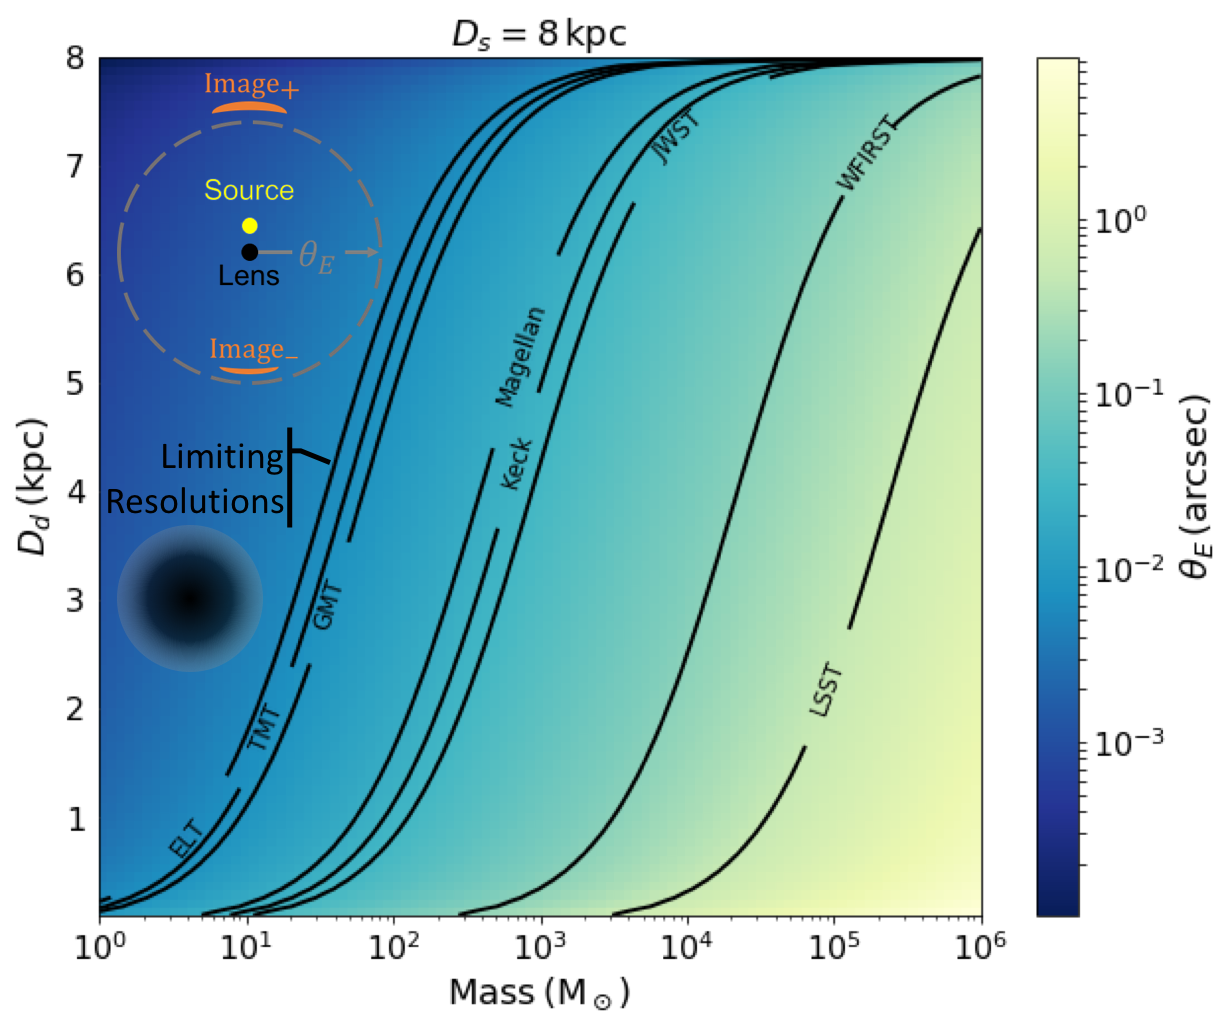
\includegraphics[width=0.6\columnwidth]{figures/StrongMicrolensing.png}
\caption{The Einstein radius (i.e., 1/2 the separation of the multiple images) for microlensing lensing events as a function of IM MACHO mass and distance between us and the MW bulge. Any parameter space below a black curve indicates that the multiple lensed source images will be resolvable by that telescope. \Contributors{Will, PALS Collaboration, ...}}
\end{figure}

% Merging Galaxy Clusters
\subsection{Merging Galaxy Clusters and Cluster Subhalos}
\Contributors{Will D., Dave W., ...}

Most dark matter constraints from merging galaxy clusters (\secref{halo_profile_clusters}) and cluster subhalos (\secref{halo_profile_clusters}) rely on accurately measuring the distribution of dark matter in (sub)clusters via gravitational lensing.
Strong and weak gravitational lensing both benefit from high resolution imaging.
For strong lensing the high resolution imaging enables better detection and characterization of strongly lensed background images in the dense cluster environment.
Similarly high resolution imaging provides $\sim4$ times more lensed source galaxies per unit area than ground-based imaging at similar depths, which enable higher resolution weak gravitational lensing.
Historically Hubble Space Telescope (HST) has provided this higher resolution imaging, although in the era of LSST it appears that we will rely on space-based telescopes such as JWST, Euclid, and WFIRST.
There is also the potential to leverage future wide field AO instruments \WAD{Need to provide and example.}.

% Strong gravitational lensing
\subsection{Strong Gravitational Lensing}
\label{sec:SLcomplement}
\Contributors{Chris F.} 

All three approaches to use strong gravitational lens systems to make inferences on the nature of dark matter that were described in \secref{stronglens} utilize LSST as a lens-finding facility.
Once the lenses are found, the dark matter science requires follow-up observations with other facilities.
The flux-ratio anomaly approach requires imaging that spatially resolves the lensed images from each other at a wavelength at which microlensing does not affect the image fluxes.
These observations can be in optical/near-IR wavelengths, utilizing IFU spectrographs behind the adaptive optics systems on ELTs to isolate the emission from the narrow-line regions of the lensed AGN, at mid-IR wavelengths with JWST, or at radio wavelengths for the subset of LSST lenses that is radio-loud.
The gravitational imaging and power-spectrum approaches both require milliarcsecond-scale angular resolution imaging for best results.
These observations require either ELT adaptive optics imaging or VLBI radio imaging of the targets.
ALMA can also be used in its most extended configuration, although this will not achieve as high a resolution as the ELTs and VLBI in most cases.

% Indirect Detection
\section{Indirect Detection }

In regions of high dark matter density, dark matter particles could continue to annihilate or decay through the same process that set their relic abundance.
Of specific interest are energetic photons (i.e., X-rays and $\gamma$ rays), since photons are produced generically by the annihilation/decay of many dark matter models (either directly or as secondarily from the production of quarks or leptons). In addition, astrophysical phenomena in extreme environments could lead to conversion between Standard Model particles and the dark sector (e.g., ALPs), which could be observable through the emission energetic photons or alterations in astrophysical spectra.
By precisely mapping the distribution of dark matter and tracking extreme events (\eg, CCSNe) LSST will enable more sensitive searches for energetic particles originating from the dark sector.

Conventional indirect detection searches focus predominantly on WIMPs with masses between several \GeV and tens of \TeV. 
The annihilation or decay of these particles could produce energetic Standard Model particles detectable by current or future experiments.
The most sensitive and robust indirect searches for dark matter rely on a precise determination of the distribution of dark matter in the universe.
The integrated flux of energetic Standard Model particles, $\phi_s$ (${\rm particles} \cm^{-2} \second^{-1}$), expected from dark matter annihilation in a density distribution, $\rho(\vect{r})$, is given by

\begin{equation}
   \phi_s(\Delta\Omega) =
    \underbrace{ \frac{1}{4\pi} \frac{\Gamma}{m_{\chi}^{a}}\int^{E_{\max}}_{E_{\min}}\frac{\text{d}N}{\text{d}E}\text{d}E}_{\rm particle\ physics}
    \cdot
    \underbrace{\vphantom{\int_{E_{\min}}} \int_{\Delta\Omega}\int_{\rm l.o.s.}\rho^{a}(\vect{r})\text{d}l\text{d}\Omega '}_{\rm astrophysics}\,.
    \label{eqn:indirect}
\end{equation}
%\Big\{\Big\}
\noindent Here, the ``particle physics'' term is strictly dependent on the particle physics properties---i.e., the particle mass, $m_\chi$,  the interaction rate, $\Gamma$, and the differential particle yield per interaction, $\text{d}N/\text{d}E$, integrated over the experimental energy range.
The second term, denoted ``astrophysics'', represents the line-of-sight integral through the dark matter distribution integrated over a solid angle, $\Delta\Omega$. 
For cases of dark matter annihilation, the interaction rate is set by the thermally averaged self-annihilation cross section, $\Gamma = \sigmav/2$, and the astrophysical integral is performed over the square of the dark matter density ($a=2$). 
The resulting astrophysical term is referred to as the ``\Jfactor'' \citep[\eg,][]{1998APh.....9..137B}. 
In cases of dark matter decay, the interaction rate is inversely proportional to the lifetime of the dark matter particle, $\Gamma = 1/\tau$, and the integral is performed over the dark matter density, $a=1$. 
The resulting term is known as the ``\Dfactor'' \citep[\eg][]{1408.0002}.
Qualitatively, the astrophysics term encapsulates the spatial distribution of the dark matter signal, while the particle physics term sets its spectral character. 
LSST will improve the sensitivity to dark matter particle physics by improving our understanding of the astrophysics term.
While these improvements will influence a wide range of indirect detection experiments, in this section we focus predominantly on $\gamma$-ray measurements.


\subsection{Milky Way Satellites \Contact{Andrew}}
\label{sec:dwarfs_id}
\Contributors{Manuel M., Esra B., Andrew P., Ethan N., Alex}

\begin{figure}[t]
\centering
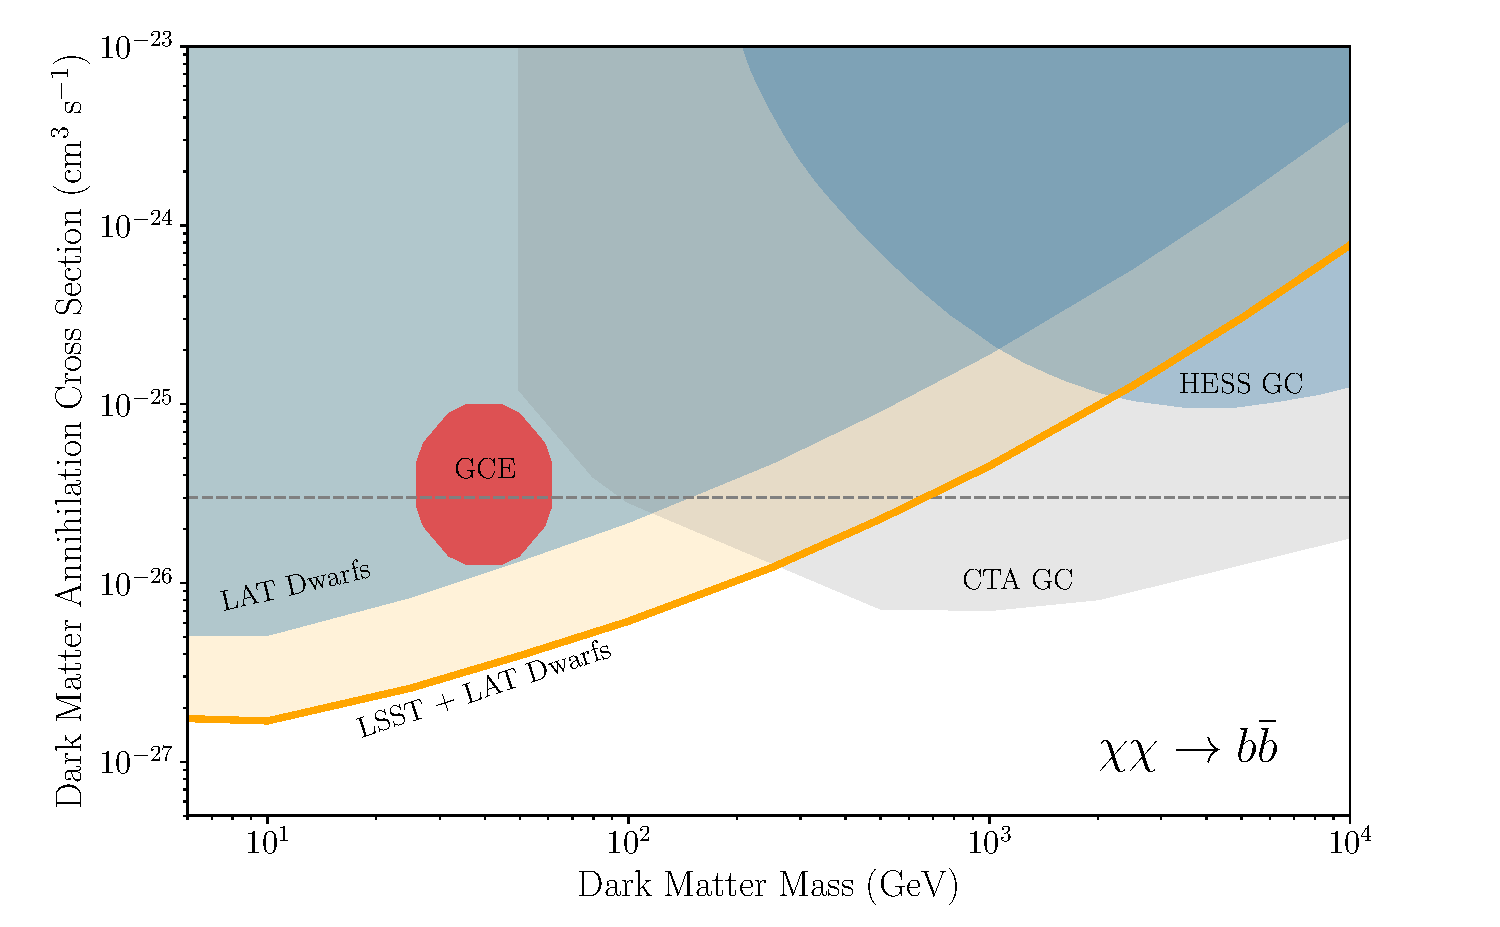
\includegraphics[width=0.75\columnwidth]{annih_limits.pdf}
\caption{Constraints on dark matter annihiltion to $b\bar{b}$ from {\it Fermi-LAT} observations of Milky Way satellite galaxies \citep[LAT Dwarfs;][]{} and HESS observations of the Galactic Center \citep[HESS GC;][]{1607.08142}. 
A bracketing range of dark matter interpretations to the  Fermi-LAT Galactic Center Excess is shown in red \citep[GCE;][]{1402.6703, Gordon:2013, Abazajian:2014}.
Projected sensitivity to dark matter annihilation combining LSST discoveries of new Milky Way satellites, improved spectroscopy of these galaxies, and continued Fermi-LAT observations is shown in gold. This projection assumes 18 years of Fermi-LAT data, a factor of 3 increase in the integrated J-factor, and a factor of 2 improvement from improved spectroscopy. 
Projected sensitivity of 500h observations of the GC with CTA are shown in gray \citep[CTA GC;][]{Zaharijas:prep}.
\label{fig:indirect}
}
\end{figure}

Gamma-ray observations of Milky Way satellite galaxies currently provide the most robust and sensitive constraints on the dark matter self-annihilation cross section for GeV- to TeV-mass particles \citep[\eg][]{Ackermann:2014, Geringer-Sameth:2015, Ackermann:2015, 1812.06986}.
The sensitivity of these searches will improve by combining new Milky Way satellite galaxies discovered by LSST, more precise \Jfactor measurements from novel spectroscopic observations, and additional Fermi-LAT data. 
We estimate each of these contributions to predict the improved sensitivity of dark matter annihilation searches in dwarf galaxies in the era of LSST.

To estimate the improvement in the integrated \Jfactor of the Milky Way satellite galaxy population, we combine cosmological zoom-in simulations of Milky Way dark matter substructure with a semi-analytic model to convert subhalo density profiles to \Jfactor estimates (this approach is is similar to that of \citealt{1309.4780}). 
Our simulation-based model accounts for modulations to dark matter-only subhalo populations due to baryonic physics, and we marginalize over the dependence of subhalo populations on host halo properties by sampling subhalo populations from a large number of hosts \citep{Nadler:2018}. 
To obtain an estimate for the increase to the integrated \Jfactor, we select a host halo with the largest number of nearby subhalos, consistent with recent observations of over-abundance of nearby satellites associated with the Milky Way \citep{Kim:2017iwr, Graus:2018}. 
We exclude subhalos with heliocentric distances $< 20 \kpc$ to avoid anomalously large projections due to a single nearby satellite.
We follow the analytic formalism presented by \citet{1604.05599} and \citet{1802.06811} to convert the dark matter profiles of our simulated subhalos to \Jfactors.  
This approach estimates the \Jfactor of each subhalo based on $r_{\max}$, $V_{\max}$, and heliocentric distance. 
%We calculate the cumulative $J$-factor within 100 kpc we find for the most optimistic case 
%(i.e., selecting the host halo with the highest cumulative $J$-factor and ignoring the effects of subhalo disruption) 
We find that the cumulative \Jfactor within 100\kpc may increase by as much as a factor of 3 relative to the known dSphs with measured \Jfactors. 

Recent studies have suggested that an additional factor of 2 improvement in sensitivity may be possible through better spectroscopic measurements  of the stars in known satellite galaxies \citep{Albert:2017}, and we include this factor in our projections.
In addition, current constraints from the Fermi-LAT Collaboration used 6 years of data \citep{Ackermann:2015}; however, the Fermi-LAT has collected more than 10 years of data and could continue to collect data for another 10+ years.
These additional data will improve the statistical sensitivity of the $\gamma$-ray search most drastically for large dark matter particle masses ($>500\GeV$).
We quantitatively evaluate the improvement from continued Fermi-LAT data taking using the results of \citep{Charles:2016}.
We combine the predicted improvements from new dwarfs, better determined \Jfactors, and more Fermi-LAT data into a projected sensitivity for future searches for dark matter annihilation in dwarf galaxies in \figref{indirect}.


\subsection{Cross correlation with gamma rays \Contact{Horiuchi,Alessandro C}}
\label{sec:igrb_id}
\Contributors{Horiuchi, Alessandro C}

Wide-area weak-lensing measurements from LSST will help extract  potential dark matter contributions to the isotropic gamma-ray background \citep[IGRB;][]{1410.3696}. The IGRB is defined as the residual all-sky $\gamma$-ray emission after subtracting individually detected sources and the Galactic diffuse emission, and provides the distance frontier of indirect dark matter searches with $\gamma$ rays. Contributions to the IGRB include unresolved sources that are individually too faint to be detected---e.g., blazars \citep{1110.3787,1310.0006}, star-forming galaxies \citep{1206.1346}, and misaligned AGNs \citep{1304.0908}---as well as a potential contribution from dark matter annihilation \citep{1312.0608,1501.05464,1501.05301,1608.07289}. Analyses of the IGRB intensity spectrum, auto-correlation angular power spectrum, and photon count statistics show that a linear combination of astrophysical sources can explain the observed IGRB, but the uncertainties are still large \citep[e.g.,][]{1502.02866}.

LSST will prove invaluable by mapping the distribution of matter on large scales via measurements of galaxy clustering and of cosmic shear from weak gravitational lensing. 
Since  cosmological $\gamma$-ray emission from dark matter annihilation follows the same underlying dark matter distribution traced by cosmic shear and galaxies, cross correlating them yields novel information on the composition of the IGRB \citep{1212.5018,1411.4651,1506.01030,Lisanti:2018,1312.4403}. 
Compared to the IGRB intensity or auto-correlation, the cross correlation will yield more than $\roughly 10$ times higher sensitivity to dark matter \citep{1411.4651,1503.05922}.
Cross-correlations with galaxy catalogs have been derived in \cite{1709.01940,1503.05918,1103.4861} up to $z \sim 0.6$ 
which is the largest redshift where current catalogs have enough sky-coverage and galaxy density to robustly
detect the correlation.  On the other hand, the IGRB is expected to extend up to $z \sim 2$--$3$ \citep{1502.02866}. 
LSST, with its large sky-coverage and galaxy density and broad redshift range, thus fills this gap to map the IGRB-LSS cross-correlation up to high redshift. 
A complete mapping of the IGRB up to $z \sim 3$ will constitute a crucial tool to robustly separate the different 
astrophysical contributions, as well as to isolate the DM annihilation signal, breaking the degeneracies which
are present when only low redshift results are used \citep{1506.01030}.    

In contrast to galaxy catalogs, cosmic shear has the advantage of being an unbiased tracer of dark matter distribution, which mitigates many of the systematics from using galaxies to trace dark matter---i.e., assumptions about the relationship between galaxy luminosity and halo mass, reliance on assumptions of hydrostatic equilibrium, and strong correlations with astrophysical $\gamma$-ray emission. At present, weak lensing surveys of several hundred square degrees allow studies of the IGRB to probe slightly above the thermal annihilation cross section \citep{1404.5503,1607.02187,1611.03554}. A simple forecast for LSST can be made by scaling the covariance matrix of the correlation estimator by the sky coverage. This shows that a combination of LSST lensing maps and all-sky Fermi-LAT data will reach a sensitivity where it is possible to \textit{detect} at $3\sigma$ WIMP annihilation to $b\bar{b}$ at the thermal cross cross section for dark matter particle masses up to 100 GeV \citep{1404.5503}.   


From the $\gamma$-ray side, improvements in the mapping of the cross-correlation with galaxies and cosmic shear are expected with the next generation of $\gamma$-ray instruments: AMEGO\footnote{\url{https://asd.gsfc.nasa.gov/amego/index.html}} and eASTROGAM\footnote{\url{http://eastrogam.iaps.inaf.it/}} \citep{1711.01265}.
At the present, the main limitation in detecting the cross-correlation at GeV and sub-GeV energies is instrumental angular resolution.  
eASTROGAM will have an angular resolution 5--6 times better than the Fermi-LAT in the energy range from $100 \MeV$ to $1 \GeV$~\citep{1711.01265}. This will translate in harmonic space into a multipole reach 5-6 times larger than presently achievable, and as a consequence stronger constraints from cross correlations.
Precise measurements of the cross-correlation at sub-GeVs will further improve the ability to separate the astrophysical IGRB sources from the DM signal, increasing the sensitivity to the latter. 

\subsection{Axion-like particle emission from supernovae \Contact{Manuel}}
\label{sec:alp_id}
\Contributors{Manuel, ...}

Axion-like particles (ALPs) might be produced during CCSNe explosions through the conversion of thermal photons in the electro-static fields of protons and ions, \ie, through the Primakoff effect \citep{1996slfp.book.....R}.  
Similar to neutrinos, ALPs would quickly escape the core and, if they are sufficiently light ($m_\phi \lesssim 10^{-9} \eV$), they could convert into $\gamma$~rays in the magnetic field of the Milky Way and/or the host galaxy of the CCSN. 
The resulting $\gamma$~rays would arrive in temporal coincidence with the neutrinos in a burst lasting tens of seconds with a 
thermal spectrum peaking 60\MeV, depending on the mass of the progenitor \citep{2015JCAP...02..006P}.
The non-observation of a $\gamma$-ray burst from the SN1987A, which occurred in the LMC, has been used to derive stringent constraints on the photon-ALP coupling $g_{\phi\gamma}<5.3\times10^{-12}\GeV^{-1}$ for $m_\phi < 4.4\times10^{-10}\eV$ \citep{1996PhLB..383..439B, 1996PhRvL..77.2372G,2015JCAP...02..006P}.
In the case of a CCSN within the Milky Way, the \textit{Fermi} LAT could improve these limits by more than an order of magnitude \citep{2017PhRvL.118a1103M}. 
However, with a Galactic supernova rate of $\roughly 3$ per century \citep[\eg,][]{2013ApJ...778..164A}, and the LAT field of view of 20\% of the sky, the chance to observe at least one such event in the next five years is $\sim 0.03 \cdot 0.2 \cdot 5 = 0.03$ (assuming that the occurrence of SNe is a Poisson process). This estimate is still optimistic since the supernova rate is calculated for the entire Galaxy, which is not inside the field of view at any given moment.\footnote{If the supernova is sufficiently nearby or the photon-ALP coupling is close to current limits, a signal could be detected with the BGO detectors (senisitive up to 40\MeV) of the \emph{Fermi} Gamma-ray Burst Monitor, which observes the entire unocculted sky.}
Increasing the search volume to extragalactic SNe is the obvious way to overcome this low rate. 
However, for CCSNe beyond the LMC and SMC, current-generation neutrino detectors lack the sensitivity to detect a signal \citep[\eg,][]{2011PhRvD..83l3008K}, and hence no precise time stamp will be provided for ALP-induced $\gamma$-ray emission; however, well-sampled optical light curves can be used to estimate the explosion time on the time scale of hours \citep{2010APh....33...19C}. 
LSST will detect a plethora of CCSNe light curves \citep{Lien:2009}. 
Estimates for the delay between the core collapse and the shock breakout range from minutes for massive Wolf-Rayet stars (type Ib/c) to days for red supergiants (type II) \citep{2013ApJ...778...81K}. 
Thus, SN type Ib/c caught early after their shock breakout and with subsequently well-sampled light curves are a prime target for the search of an ALP-induced $\gamma$-ray burst. 

Since the $\gamma$-ray flux scales as $g_{\phi\gamma}^4 / d^2$, where $d$ is the luminosity distance, the sensitivity for $g_{\phi\gamma}$ scales as $\sqrt{d}$. 
Limits of the order of $g_{\phi\gamma} \lesssim 2\times10^{-12}\,\mathrm{GeV}^{-1}$ should be possible for a single supernova in M31 ($d=778\kpc$) \citep{2017PhRvL.118a1103M}. 
If one allows these limits to degrade by a factor of 10, constraints better than those from CAST should still be possible for $d\lesssim 80\Mpc$ ($z \lesssim 0.02$) for a single SN assuming that the time of the core collapse is precisely known. 
LSST is expected to detect tens of type Ib/c CCSNe each year with redshifts $z \lesssim 0.02$ \citep{Goldstein:2018} and could conduct such searches in conjunction with the \textit{Fermi} satellite or future $\gamma$-ray satellites like AMEGO, eASTROGAM, or Gamma-400 \citep[\eg,][]{2017ICRC...35..910C,1502.02976} 
A stacking analysis of the $\gamma$-ray data with explosions times estimated from LSST light curves provides the exciting possibility to photon-ALP couplings in the regime where ALPs could make up the entirety of the dark matter. 


% Direct Detection
\section{Direct Detection }
\ADW{Some introduction and context is needed here. Much of Lina's intro could be moved here.}

\subsection{Baryon Scattering \Contact{Vera}}
\Contributors{Vera, Kim, Lina N.}

The most sensitive low-energy searches for dark matter are looking to directly detect collisions of dark matter particles from the local galactic halo in underground detectors \citep{2013arXiv1310.8327C}. 
They have unprecedented sensitivity to WIMPs with masses well above a GeV, but the current generation of experiments is largely insensitive to lighter particles, for kinematic reasons. 
New technologies are necessary to open up sub-GeV models of dark matter to detailed exploration \citep{Battaglieri:2017aum}. 
Moreover, due to the extensive shielding of their targets, direct detection experiments have a ceiling on their sensitivity to large cross sections. 
The portion of dark matter parameter space excluded by current null results is shown in \figref{dd}. 
\begin{figure}
\centering
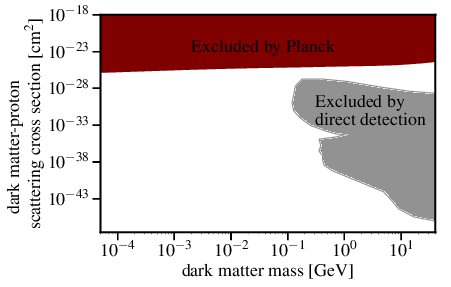
\includegraphics[width=0.6\columnwidth]{figures/planck_dd.png}
\caption{Currently-excluded regions of dark matter parameter space (mass versus cross section for scattering with protons through a velocity-independent spin-independent contact interaction) are shown as shaded regions. Gray region is excluded by various direct detection null results \citep{2018PhRvD..97l3013K} and red is excluded by CMB measurements \citep{Gluscevic:2017ywp}. We note that there are other limits in the same parameter space, but we choose to compare only these two, for illustration of complementarity between cosmological and low-energy laboratory searches.}
\label{fig:dd}
\end{figure}

Current null results from targeted laboratory searches motivate broad scans of parameter space that is inaccessible to underground experiments. Cosmological and astrophysical observables provide such a complementary search strategy. In particular, they are sensitive to scattering of sub-GeV particles with baryons at any point in cosmic history. Furthermore, there is no upper boundary on the interaction cross section they can probe. Finally, they are not subject to the uncertainty on local astrophysical properties of dark matter particles (their phase-space distribution), which affects the inferred limits on the particle properties of dark matter. 

If dark matter particles scatter with baryons, they transfer momentum between the two cosmological fluids, affecting density fluctuations and suppressing power at small scales; the power suppression can be captured by a variety of observables. The current limits come from the CMB \citep{Gluscevic:2017ywp}, cosmic-ray \citep{Cappiello:2018hsu}, and Lyman-$\alpha$ forest measurements \cite{Xu:2018efh}. For illustration, Figure \ref{fig:dd} compares currently excluded regions of dark matter parameter space, from analyses of Planck data, and from null results of various direct-detection searches.\footnote{We caution the reader that this is not a comprehensive list of current upper limits, but only serves to illustrate complementarity of cosmological and direct detection probes.} LSST will deliver state-of-the-art measurements of observables that trace matter fluctuations on a range of smaller scales, extending the sensitivity of astrophysical and cosmological searches far beyond the reach of Planck.

\subsection{Local Dark Matter Velocity Distribution \Contact{Lina}}
\Contributors{Lina N.}

%One way to detect dark matter (DM) is a process called direct detection, where DM particles scatter off heavy nuclei, emitting scintillation/ionization light that provide a direct signal of DM \citep{Goodman:1984dc}. 

The signal strength of dark matter (DM) scattering in direct detection experiments depends on both the local DM density and the DM velocity distribution. In this section we focus on the DM velocity distribution.

The differential rate with respect to the recoil energy $dR/dQ$ depends on the integral of the DM velocity distribution, $f(v)$, as
\begin{equation}
    \frac{dR}{dQ} \propto \int_{v_{\rm{min}}}^{v_{\rm{esc}}} \frac{f(v)}{v} dv, 
\end{equation}
where $v_{\rm{min}} = \sqrt{Q m_N/ (2 \mu^2)}$, with $Q$ the recoil energy, $m_N$ the mass of the nucleus against which DM is scattering, and $\mu = (m_N m_\chi / (m_N + m_\chi))$ the reduced mass of the nucleus $m_N$ and the DM mass $m_\chi$.

A novel method has recently been proposed to use the stars as tracers for the DM velocity \citep{Herzog-Arbeitman:2017fte,Necib:2018b}. These papers suggest that since accreted DM and stars have a comment origin, and are both collisionless, accreted stars are able to trace the velocity distribution of DM. This correlation holds for both the relaxed component of the DM, traced by older metal poor stars, and DM velocity substructure called debris flow traced by less metal poor stars from more recent mergers \citep{Lisanti:2011as,Kuhlen:2012fz,Lisanti:2014dva}. 

This method has already been applied on RAVE-TGAS data \citep{Herzog-Arbeitman:2017zbm}, and the second data release of Gaia in \cite{necib2018}. It has been found that the relaxed component of the DM although isotropic, has a mean speed lower than that of the assumed Maxwell Boltzmann distribution, reducing current limits by direct detection experiments \citep{Aprile:2018dbl}.

Another interesting aspect is the ability to reconstruct of more recent mergers. Using the second data release of Gaia, a new merger called the Gaia Sausage or the Gaia Enceleadus \citep{2018MNRAS.477.1472B,2018Natur.563...85H} has been found. Using the correlation observed in simulations, \cite{necib2018} extracted the new velocity distribution of DM brought in by the same merger, and studied its implications in current direct detection experiments. 

In order to do obtain the full empirical distribution of DM, one needs the 3-d velocities of the stars in the local neighborhood. Gaia provides proper motion and parallaxes for stars down to 20th magnitude. LSST will be able to extend this dataset to fainter stars, giving us a more accurate measurement of proper motions of stars in the solar neighborhood and beyond.

 Using proper motions of stars from LSST, coupled with radial velocity measurements from future telescopes like MSE, we will be able to obtain the most accurate 3-d velocity measurements of the local stars, and subsequently use this information to obtain a full empirical measurement of DM. Such detailed analysis will unveil new structures much smaller than the Gaia Sausage, but with equal importance in DM direct detection if it passes by the Solar neighborhood.



\begin{comment}
\bsection{Particle Accelerators \Contact{???}}
\Contributors{...}
\ADW{If no one steps up here, we should remove this section.}
\end{comment}

\begin{comment}
\section{Cosmic Microwave Background \Contributors{Vera,Kim,Francis-Yan,Cora}}

Consider removing this section for now. Points to potentially consider in the future:
\begin{itemize}
    \item Cross-correlation science.
    \item CMB limits on dark matter-baryon and dark matter-dark radiation interactions are robust, but probe large scales. Smaller-scale probes (dwarfs etc) have a better discovery potential.
    \item In a meta-analysis where many observables are fit with all parameters of interest, we'd want to vary all LCDM parameters. We'd use CMB data for this, in a joint likelihood analysis. But we're not there yet.
\end{itemize}
\end{comment}

\begin{comment}
\subsection{Gravitational Waves \Contact{???}}
\Contributors{...}
\ADW{If no one steps up here, we should remove this section.}
\end{comment}

\begin{comment}
\subsection{Radio \Contact{Will?}}
\Contributors{Will, Tony, ...}
\label{sec:radio} 

% Radio Relics: SKA, etc.
\WAD{Need to flesh out this section.}
\begin{itemize}
    \item Radio relics are...
    \item Because radio relics are only associated with post-major-cluster-mergers they can be a convenient way of identifying post-mergers.
    \item Given the spectral index ($\alpha\sim-2$) radio relics are easier to detect at frequencies of order 100 MHz.
    \item In the era of LSST, SKA will provide the best means of detecting mergers through their radio relics
    \item According to \cite{2012MNRAS.420.2006N} LOFAR will detect $\sim2500$ radio relics. Given that SKA will be XXX times more sensitive it can be expected to detect YYY radio relics in the southern hemisphere. \WAD{Need to scale the sensitivity to estimate the number of relics that will be detected.}
\end{itemize}
\end{comment}

\begin{comment}
\subsection{X-Ray \Contact{???}}
\Contributors{Will, Tony, Esra, ...}
\label{sec:xray} 
% LSST plus X-ray facilities: etc.
{\color{red} Esra will write a section on eROSITA and Athena complementary X-ray observations here. This section can also be moved to Galaxy clusters section}

\begin{itemize}
    \item Given Athena's all sky coverage and resolution it should provide the necessary course spatial and spectral characterization of gas and merging clusters.
\end{itemize}
\end{comment}

\begin{comment}
\subsection{Targeted Follow Up \Contact{???}}
\Contributors{Nate, Will, Michael...}
\subsubsection{Transients}
\end{comment}
